\documentclass[10pt,a4paper]{article}
\usepackage{tocloft}
\usepackage{commons/course}  % همین کافیه؛ listings و xcolor داخلشه
\usepackage{booktabs}
\usepackage{longtable}
\usepackage{float}

% Define colors for syntax highlighting
\definecolor{keywordstyle}{rgb}{0.0, 0.4, 0.8}
\definecolor{stringstyle}{rgb}{0.9, 0.17, 0.31}
\definecolor{commentstyle}{rgb}{0.1, 0.6, 0.2}
\definecolor{numberstyle}{rgb}{0.4, 0.4, 0.4}
\definecolor{backgroundcolor}{rgb}{0.94, 0.97, 1.0}

\lstdefinelanguage{PythonLike}{
	morekeywords={mov, add, sub, cmp, jmp , lw , addi,sw,bne},
	sensitive=false,
	morecomment=[l]{;},
	morestring=[b]",
}

\lstset{
	language=PythonLike,
	basicstyle=\ttfamily\small,
	keywordstyle=\color{keywordstyle},
	stringstyle=\color{stringstyle},
	commentstyle=\color{commentstyle},
	numbers=left,
	numberstyle=\tiny\color{numberstyle},
	stepnumber=1,
	numbersep=5pt,
	keepspaces=true,
	tabsize=4,
	showspaces=false,
	showstringspaces=false,
	showtabs=false,
	breaklines=true,
	breakatwhitespace=false,
	frame=single,
	backgroundcolor=\color{backgroundcolor},
}

\newlistof{listofproblems}{lop}{\normalsize فهرست مسائل}
\newcommand{\addproblem}[1]{\addcontentsline{lop}{listofproblems}{\protect\numberline{}#1}}


\begin{document}


\سربرگ{آزمایش پنجم}{تبدیل عدد دهدهی به دودویی}{معین آعلی - ثمین اکبری}{استاد: دکتر حمید سربازی آزاد}

\subsubsection*{خلاصه}

در این آزمایش مداری طراحی شده که یک عدد دهدهی سه‌رقمی به فرم \lr{BCD} را می‌گیرد و با فعال‌شدن سیگنال \lr{Start} آن را به معادل دودویی تبدیل می‌کند و در پایان سیگنال \lr{End} را فعال می‌کند. 
تراشه‌های استفاده شده: شش عدد \lr{74194} به‌عنوان ثبات‌های ارقام و ثبات نتیجه، سه عدد \lr{74283} برای عمل تصحیح تفریق ۳، سه عدد \lr{74157} برای انتخاب مسیر داده، یک \lr{74161} برای شمارش تکرارها، و \lr{7404}، \lr{7408} و \lr{7432} برای واحد کنترل. مجموعا ۱۶ تراشه.



% ============================ عکس بلوک دیاگرام ============================
\subsubsection*{بلوک دیاگرام مدار}
\begin{figure}[h]
  \centering
  
\includegraphics[width=0.3\textwidth]{figs/block.png}
\end{figure}


\subsubsection*{هدف آزمایش}

هدف، طراحی مداری است که عدد دهدهی سه‌رقمی را به معادل دودویی تبدیل کند. اهداف مشخص عبارت‌اند از:

\begin{itemize}
  \item آشنایی عملی با الگوریتم تبدیل \lr{BCD} به دودویی به روش شیفت راست و تفریق ۳ (معکوس \lr{Double Dabble}).
  \item پیاده‌سازی مدار با تراشه‌های استاندارد \lr{TTL} سری ۷۴، بدون استفاده از ماژول‌های آماده‌ی تبدیل.
  \item طراحی واحد کنترل ترتیبی با سیگنال‌های \lr{Start} و \lr{End}.
  \item بررسی صحت عملکرد با پوشش کامل هر ۱۰۰۰ ورودی ممکن.
\end{itemize}


\subsubsection*{رابط مدار}

مدار اصلی \lr{converter} است و مدار \lr{main} همان را برای نمایش با \lr{Clock} و نمایشگرهای هفت‌قطعه‌ای می‌پیچد.

\begin{center}
\begin{tabular}{@{}llll@{}}
\toprule
{سیگنال} & {جهت} & {پهنا} & {توضیح} \\
\midrule
\lr{A} & ورودی & ۱۲ & عدد \lr{BCD}: $A[11{:}8]$ صدگان، $A[7{:}4]$ دهگان، $A[3{:}0]$ یکان \\
\lr{Start} & ورودی & ۱ & سطحی؛ شروع عملیات \\
\lr{clk} & ورودی & ۱ & لبه‌ی بالارونده \\
\lr{B} & خروجی & ۱۰ & معادل دودویی (۰ تا ۹۹۹) \\
\lr{End} & خروجی & ۱ & با معتبرشدن \lr{B} فعال می‌شود \\
\bottomrule
\end{tabular}
\end{center}

خروجی ۱۰ بیت است چون بزرگ‌ترین ورودی یعنی ۹۹۹ برابر $(1111100111)_2$ می‌شود که ۱۰ بیت لازم دارد.

در مدار \lr{main} به‌جای یک ورودی ۱۲ بیتی، سه ورودی ۴ بیتی مجزا (\lr{A2}، \lr{A1}، \lr{A0}) گرفته می‌شود تا هر رقم روی نمایشگر خودش دیده شود.


\subsubsection*{الگوریتم تبدیل}

طبق دستور کار، الگوریتم تبدیل یک عدد دهدهی $r$ رقمی به دودویی معادل به این صورت است:

\begin{enumerate}
  \item[الف)] عدد دهدهی ورودی را یک بیت به راست شیفت بده.
  \item[ب)] اگر باارزش‌ترین بیت رقم $i$ام یک باشد، از آن رقم ۳ واحد کم کن.
  \item[ج)] مراحل الف و ب را تا زمانی که تمام ارقام دهدهی صفر شوند تکرار کن (حداکثر ۱۰ بار).
\end{enumerate}

بیت‌هایی که با شیفت به راست از سمت کم‌ارزش بیرون می‌آیند، به ترتیب عدد دودویی معادل را تشکیل می‌دهند.

{چرا این الگوریتم کار می‌کند؟} شیفت راست یعنی تقسیم بر ۲. اما در نمایش \lr{BCD} هر رقم وزن ۱۰ دارد نه ۱۶. وقتی بیتی از یک رقم به رقم پایین‌تر منتقل می‌شود، به‌جای ارزش ۱۰ ارزش ۱۶ پیدا می‌کند، یعنی ۶ واحد اضافه‌تر. چون این خطا بعد از شیفت (یعنی تقسیم بر ۲) دیده می‌شود، مقدار تصحیح نصف ۶ یعنی ۳ است. بنابراین هر رقمی که بعد از شیفت مقدارش از ۷ بیشتر شود (یعنی پرارزش‌ترین بیتش ۱ شود) باید ۳ واحد کم کند.

{تعداد تکرار.} چون خروجی ۱۰ بیت است، دقیقا ۱۰ تکرار لازم است. در پیاده‌سازی، به‌جای تشخیص همه‌ی ارقام صفر شدند از یک شمارنده‌ی ثابت ۱۰ تایی استفاده شده که هم ساده‌تر است و هم زمان اجرا را قطعی می‌کند.

\vspace{0.5em}
تریس برای ورودی $A = 999$:

\begin{LTR}
\begin{center}
\begin{tabular}{@{}ccccl@{}}
\toprule
iteration & hundreds & tens & units & binary register \\
\midrule
init & 9 & 9 & 9 & \lr{00 0000 0000} \\
1  & 4 & 9 & 9 & \lr{10 0000 0000} \\
2  & 2 & 4 & 9 & \lr{11 0000 0000} \\
3  & 1 & 2 & 4 & \lr{11 1000 0000} \\
4  & 0 & 6 & 2 & \lr{01 1100 0000} \\
5  & 0 & 3 & 1 & \lr{00 1110 0000} \\
6  & 0 & 1 & 5 & \lr{10 0111 0000} \\
7  & 0 & 0 & 7 & \lr{11 0011 1000} \\
8  & 0 & 0 & 3 & \lr{11 1001 1100} \\
9  & 0 & 0 & 1 & \lr{11 1100 1110} \\
10 & 0 & 0 & 0 & \lr{11 1110 0111} \\
\bottomrule
\end{tabular}
\end{center}
\end{LTR}

نتیجه $(1111100111)_2 = 999$ که درست است. توجه کنید در پایان هر سه رقم صفر شده‌اند، که نشانه‌ی درستی کار است.

\vspace{0.5em}
برای نمونه، در تکرار ۱ رقم صدگان: ابتدا $9 = (1001)_2$ یک بیت به راست شیفت می‌شود و چون از بالا صفر وارد می‌شود $(0100)_2 = 4$ به دست می‌آید. پرارزش‌ترین بیت آن صفر است پس تصحیح لازم ندارد. اما در تکرار ۴ رقم دهگان بعد از شیفت $(1001)_2 = 9$ می‌شود؛ چون بیت سوم آن یک است، $9 - 3 = 6$ می‌شود که در جدول دیده می‌شود.


\subsubsection*{فرمول‌بندی سخت‌افزاری}

برای پیاده‌سازی، الگوریتم به این شکل بازنویسی شده که هر تکرار دقیقا یک سیکل ساعت طول بکشد. ثبات هر رقم همیشه مقدار {تصحیح‌شده} را نگه می‌دارد؛ شیفت با سیم‌کشی و تصحیح با جمع‌کننده انجام می‌شود:

\[
\begin{aligned}
\mathrm{shifted}_k &= (D_k \gg 1) \;|\; (s_k \ll 3) \\
D_k(\text{next}) &= \mathrm{shifted}_k + (\mathrm{shifted}_k[3] \;?\; 13 : 0)
\end{aligned}
\]

که در آن $s_k$ بیتی است که از رقم باارزش‌تر وارد می‌شود:
\[
s_{\text{صدگان}} = 0, \qquad
s_{\text{دهگان}} = D_{\text{صدگان}}[0], \qquad
s_{\text{یکان}} = D_{\text{دهگان}}[0]
\]

{چرا جمع ۱۳؟} در حساب پیمانه‌ی ۱۶، تفریق ۳ با جمع متمم دوی آن یعنی $16 - 3 = 13 = (1101)_2$ برابر است. پس به‌جای مدار تفریق، یک جمع‌کننده‌ی \lr{74283} کافی است که ورودی دومش وقتی تصحیح لازم است $(1101)_2$ باشد و در غیر این صورت صفر.

 پرارزش‌ترین بیت مقدار \emph{شیفت‌شده} دقیقا همان بیت $s_k$ است که از رقم بالاتر وارد شده است. یعنی شرط تصحیح از قبل به‌صورت یک سیم در دسترس است و لازم نیست با گیت ساخته شود. بنابراین ورودی دوم جمع‌کننده به این صورت سیم می‌شود:

\begin{center}
\begin{tabular}{@{}ll@{}}
\toprule
{ورودی جمع‌کننده} & {به چه وصل است} \\
\midrule
$A_4\,A_3\,A_2\,A_1$ & $s_k,\; b_3,\; b_2,\; b_1$ \quad (رقم شیفت‌خورده) \\
$B_4\,B_3\,B_2\,B_1$ & $s_k,\; s_k,\; \mathrm{GND},\; s_k$ \quad (وقتی $s_k=1$ مقدار $(1101)_2=13$) \\
$C_{in}$ & \lr{GND} \\
\bottomrule
\end{tabular}
\end{center}

چون $s_k$ خودش خروجی $Q$ یک ثبات دیگر است، {کل عمل تصحیح تفریق ۳ هیچ گیت اضافه‌ای مصرف نمی‌کند} و فقط سه پین جمع‌کننده به همان سیم وصل می‌شوند. این مهم‌ترین بهینه‌سازی این طراحی است.


\subsubsection*{معماری کلی}

هر رقم \lr{BCD} یک برش دارد که از سه تراشه تشکیل شده است:

\begin{center}
\begin{tabular}{@{}ll@{}}
\toprule
{تراشه} & {کار} \\
\midrule
\lr{74194} & ثبات نگهدارنده‌ی رقم؛ هر سیکل بارگذاری موازی می‌شود \\
\lr{74283} & شیفت راست و تصحیح تفریق ۳ (کاملا ترکیبی) \\
\lr{74157} & انتخاب می‌کند: هنگام \lr{Start} مقدار ورودی، در غیر این صورت مقدار تصحیح‌شده \\
\bottomrule
\end{tabular}
\end{center}

مسیر داده در هر برش یک حلقه است:

 خروجی ثبات $\rightarrow$ جمع‌کننده $\rightarrow$ مالتی‌پلکسر $\rightarrow$ ورودی ثبات
 
 بیت کم‌ارزش هر رقم به‌عنوان ورودی سریال به برش پایین‌تر می‌رود، و بیت کم‌ارزش رقم یکان وارد ثبات نتیجه می‌شود.

\vspace{0.5em}
جدول کامل تراشه‌ها:

\begin{center}
\begin{tabular}{@{}lll@{}}
\toprule
{مرجع} & {تراشه} & {نقش} \\
\midrule
\lr{U1} & \lr{74194} & ثبات رقم صدگان \\
\lr{U2} & \lr{74194} & ثبات رقم دهگان \\
\lr{U3} & \lr{74194} & ثبات رقم یکان \\
\lr{U4} & \lr{74283} & شیفت و تصحیح رقم صدگان \\
\lr{U5} & \lr{74283} & شیفت و تصحیح رقم دهگان \\
\lr{U6} & \lr{74283} & شیفت و تصحیح رقم یکان \\
\lr{U7} & \lr{74157} & انتخاب منبع رقم صدگان \\
\lr{U8} & \lr{74157} & انتخاب منبع رقم دهگان \\
\lr{U9} & \lr{74157} & انتخاب منبع رقم یکان \\
\lr{U10} & \lr{74194} & ثبات نتیجه، بیت‌های $B[9{:}6]$ \\
\lr{U11} & \lr{74194} & ثبات نتیجه، بیت‌های $B[5{:}2]$ \\
\lr{U12} & \lr{74194} & ثبات نتیجه، بیت‌های $B[1{:}0]$ \\
\lr{U13} & \lr{74161} & شمارنده‌ی تکرار، تا ۱۰ می‌شمارد \\
\lr{U14} & \lr{7404} & اینورتر: تولید \lr{nCLR} و \lr{RUN} \\
\lr{U15} & \lr{7408} & گیت \lr{AND}: تشخیص رسیدن شمارنده به ۱۰ \\
\lr{U16} & \lr{7432} & گیت \lr{OR}: تولید سیگنال \lr{LD} \\
\bottomrule
\end{tabular}
\end{center}


\subsubsection*{واحد کنترل}

واحد کنترل تنها از سه گیت استفاده می‌کند:

\[
\begin{aligned}
\mathrm{nCLR} &= \mathrm{NOT}(\mathrm{Start}) && \text{(از \lr{U14})} \\
\mathrm{RUN}  &= \mathrm{NOT}(\mathrm{End})   && \text{(از \lr{U14})} \\
\mathrm{End}  &= \mathrm{Cq3} \cdot \mathrm{Cq1} && \text{(از \lr{U15})} \\
\mathrm{LD}   &= \mathrm{Start} + \mathrm{RUN} && \text{(از \lr{U16})}
\end{aligned}
\]

سیگنال \lr{End} وقتی فعال می‌شود که شمارنده به مقدار $10 = (1010)_2$ برسد، یعنی بیت‌های ۳ و ۱ آن هم‌زمان یک باشند. سیگنال \lr{LD} باعث می‌شود ثبات ارقام هم در فاز بارگذاری و هم در فاز اجرا مقدار بگیرد، ولی بعد از پایان کار مقدار خود را نگه دارد.

\vspace{0.5em}
جدول فازهای کاری:

\begin{center}
\begin{tabular}{@{}lllllll@{}}
\toprule
{فاز} & \lr{Start} & \lr{End} & \lr{LD} & {ثبات ارقام} & {ثبات نتیجه} & {شمارنده} \\
\midrule
بارگذاری & ۱ & ۰ & ۱ & بارگذاری \lr{A} & پاک با \lr{nCLR} & پاک با \lr{nCLR} \\
اجرا & ۰ & ۰ & ۱ & بارگذاری تصحیح‌شده & شیفت راست & می‌شمارد \\
پایان & ۰ & ۱ & ۰ & نگه‌داری & نگه‌داری & ثابت روی ۱۰ \\
\bottomrule
\end{tabular}
\end{center}

کدگذاری مد \lr{74194} روی پین‌های $S_1 S_0$: مقدار \lr{11} بارگذاری موازی، \lr{01} شیفت راست، و \lr{00} نگه‌داری است. ثبات‌های ارقام هر دو پین را به \lr{LD} وصل کرده‌اند (پس یا بارگذاری یا نگه‌داری) و ثبات‌های نتیجه $S_1 = \mathrm{GND}$ و $S_0 = \mathrm{RUN}$ دارند (پس یا شیفت راست یا نگه‌داری).


\subsubsection*{جزئیات پایه‌های تراشه‌ها}
در این بخش برای هر تراشه، شماره‌ی پین، نام آن طبق دیتاشیت، و سیگنالی که به آن وصل شده آورده شده است. پین‌های تغذیه (\lr{VCC} و \lr{GND}) در لاجسیم پورت ندارند ولی برای کامل بودن جدول ذکر شده‌اند.

\paragraph{ثبات‌های ارقام \lr{BCD}}\mbox{}\\
هر سه یکسان سیم‌کشی شده‌اند و فقط نام سیگنال‌هایشان فرق می‌کند. پین‌های $S_1$ و $S_0$ هر دو به \lr{LD} وصل‌اند، پس ثبات یا بارگذاری موازی می‌کند یا مقدار را نگه می‌دارد. پین \lr{nCLR} به \lr{VCC} بسته شده چون مقداردهی اولیه از راه مالتی‌پلکسر انجام می‌شود نه پاک‌سازی. در \lr{74194} پین \lr{QA} پرارزش‌ترین بیت و \lr{QD} کم‌ارزش‌ترین است.

\begin{center}
\small
{\lr{U1} — \lr{74194} — ثبات رقم صدگان}

\begin{tabular}{@{}clll@{}}
\toprule
{پین} & {نام} & {سیگنال} & {توضیح} \\
\midrule
1 & \lr{nCLR} & \lr{VCC} & سطح منطقی ۱ \\
2 & \lr{SR} & \lr{GND} & سطح منطقی ۰ \\
3 & \lr{A} & \lr{D2m3} & بیت 3 خروجی مالتی‌پلکسر \\
4 & \lr{B} & \lr{D2m2} & بیت 2 خروجی مالتی‌پلکسر \\
5 & \lr{C} & \lr{D2m1} & بیت 1 خروجی مالتی‌پلکسر \\
6 & \lr{D} & \lr{D2m0} & بیت 0 خروجی مالتی‌پلکسر \\
7 & \lr{SL} & \lr{GND} & سطح منطقی ۰ \\
8 & \lr{GND} & \lr{GND} & سطح منطقی ۰ \\
9 & \lr{S0} & \lr{LD} & بارگذاری ( Start + RUN ) \\
10 & \lr{S1} & \lr{LD} & بارگذاری ( Start + RUN ) \\
11 & \lr{CLK} & \lr{CLK} & ساعت مدار \\
12 & \lr{QD} & \lr{D2b0} & بیت 0 رقم صدگان (خروجی ثبات) \\
13 & \lr{QC} & \lr{D2b1} & بیت 1 رقم صدگان (خروجی ثبات) \\
14 & \lr{QB} & \lr{D2b2} & بیت 2 رقم صدگان (خروجی ثبات) \\
15 & \lr{QA} & \lr{D2b3} & بیت 3 رقم صدگان (خروجی ثبات) \\
16 & \lr{VCC} & \lr{VCC} & سطح منطقی ۱ \\
\bottomrule
\end{tabular}
\end{center}

\begin{center}
\small
{\lr{U2} — \lr{74194} — ثبات رقم دهگان}

\begin{tabular}{@{}clll@{}}
\toprule
{پین} & {نام} & {سیگنال} & {توضیح} \\
\midrule
1 & \lr{nCLR} & \lr{VCC} & سطح منطقی ۱ \\
2 & \lr{SR} & \lr{GND} & سطح منطقی ۰ \\
3 & \lr{A} & \lr{D1m3} & بیت 3 خروجی مالتی‌پلکسر \\
4 & \lr{B} & \lr{D1m2} & بیت 2 خروجی مالتی‌پلکسر \\
5 & \lr{C} & \lr{D1m1} & بیت 1 خروجی مالتی‌پلکسر \\
6 & \lr{D} & \lr{D1m0} & بیت 0 خروجی مالتی‌پلکسر \\
7 & \lr{SL} & \lr{GND} & سطح منطقی ۰ \\
8 & \lr{GND} & \lr{GND} & سطح منطقی ۰ \\
9 & \lr{S0} & \lr{LD} & بارگذاری ( Start + RUN ) \\
10 & \lr{S1} & \lr{LD} & بارگذاری ( Start + RUN ) \\
11 & \lr{CLK} & \lr{CLK} & ساعت مدار \\
12 & \lr{QD} & \lr{D1b0} & بیت 0 رقم دهگان (خروجی ثبات) \\
13 & \lr{QC} & \lr{D1b1} & بیت 1 رقم دهگان (خروجی ثبات) \\
14 & \lr{QB} & \lr{D1b2} & بیت 2 رقم دهگان (خروجی ثبات) \\
15 & \lr{QA} & \lr{D1b3} & بیت 3 رقم دهگان (خروجی ثبات) \\
16 & \lr{VCC} & \lr{VCC} & سطح منطقی ۱ \\
\bottomrule
\end{tabular}
\end{center}

\begin{center}
\small
{\lr{U3} — \lr{74194} — ثبات رقم یکان}

\begin{tabular}{@{}clll@{}}
\toprule
{پین} & {نام} & {سیگنال} & {توضیح} \\
\midrule
1 & \lr{nCLR} & \lr{VCC} & سطح منطقی ۱ \\
2 & \lr{SR} & \lr{GND} & سطح منطقی ۰ \\
3 & \lr{A} & \lr{D0m3} & بیت 3 خروجی مالتی‌پلکسر \\
4 & \lr{B} & \lr{D0m2} & بیت 2 خروجی مالتی‌پلکسر \\
5 & \lr{C} & \lr{D0m1} & بیت 1 خروجی مالتی‌پلکسر \\
6 & \lr{D} & \lr{D0m0} & بیت 0 خروجی مالتی‌پلکسر \\
7 & \lr{SL} & \lr{GND} & سطح منطقی ۰ \\
8 & \lr{GND} & \lr{GND} & سطح منطقی ۰ \\
9 & \lr{S0} & \lr{LD} & بارگذاری ( Start + RUN ) \\
10 & \lr{S1} & \lr{LD} & بارگذاری ( Start + RUN ) \\
11 & \lr{CLK} & \lr{CLK} & ساعت مدار \\
12 & \lr{QD} & \lr{D0b0} & بیت 0 رقم یکان (خروجی ثبات) \\
13 & \lr{QC} & \lr{D0b1} & بیت 1 رقم یکان (خروجی ثبات) \\
14 & \lr{QB} & \lr{D0b2} & بیت 2 رقم یکان (خروجی ثبات) \\
15 & \lr{QA} & \lr{D0b3} & بیت 3 رقم یکان (خروجی ثبات) \\
16 & \lr{VCC} & \lr{VCC} & سطح منطقی ۱ \\
\bottomrule
\end{tabular}
\end{center}

\paragraph{جمع‌کننده‌های تصحیح}\mbox{}\\
ورودی $A$ همان رقم شیفت‌خورده است و ورودی $B$ مقدار $(1101)_2=13$ را وقتی تصحیح لازم است می‌سازد. دقت کنید در \lr{U4} (صدگان) چون بیت ورودی همیشه صفر است، تمام ورودی‌های $B$ به \lr{GND} بسته شده‌اند؛ یعنی رقم صدگان هرگز تصحیح نمی‌خواهد. پین \lr{Cout} استفاده نمی‌شود چون نتیجه همیشه در ۴ بیت جا می‌شود.

\begin{center}
\small
{\lr{U4} — \lr{74283} — شیفت و تصحیح رقم صدگان}

\begin{tabular}{@{}clll@{}}
\toprule
{پین} & {نام} & {سیگنال} & {توضیح} \\
\midrule
1 & \lr{S2} & \lr{D2n1} & بیت 1 مقدار تصحیح‌شده \\
2 & \lr{B2} & \lr{GND} & سطح منطقی ۰ \\
3 & \lr{A2} & \lr{D2b2} & بیت 2 رقم صدگان (خروجی ثبات) \\
4 & \lr{S1} & \lr{D2n0} & بیت 0 مقدار تصحیح‌شده \\
5 & \lr{A1} & \lr{D2b1} & بیت 1 رقم صدگان (خروجی ثبات) \\
6 & \lr{B1} & \lr{GND} & سطح منطقی ۰ \\
7 & \lr{Cin} & \lr{GND} & سطح منطقی ۰ \\
8 & \lr{GND} & \lr{GND} & سطح منطقی ۰ \\
9 & \lr{Cout} & \lr{---} & بدون اتصال \\
10 & \lr{S4} & \lr{D2n3} & بیت 3 مقدار تصحیح‌شده \\
11 & \lr{B4} & \lr{GND} & سطح منطقی ۰ \\
12 & \lr{A4} & \lr{GND} & سطح منطقی ۰ \\
13 & \lr{S3} & \lr{D2n2} & بیت 2 مقدار تصحیح‌شده \\
14 & \lr{A3} & \lr{D2b3} & بیت 3 رقم صدگان (خروجی ثبات) \\
15 & \lr{B3} & \lr{GND} & سطح منطقی ۰ \\
16 & \lr{VCC} & \lr{VCC} & سطح منطقی ۱ \\
\bottomrule
\end{tabular}
\end{center}

\begin{center}
\small
{\lr{U5} — \lr{74283} — شیفت و تصحیح رقم دهگان}

\begin{tabular}{@{}clll@{}}
\toprule
{پین} & {نام} & {سیگنال} & {توضیح} \\
\midrule
1 & \lr{S2} & \lr{D1n1} & بیت 1 مقدار تصحیح‌شده \\
2 & \lr{B2} & \lr{GND} & سطح منطقی ۰ \\
3 & \lr{A2} & \lr{D1b2} & بیت 2 رقم دهگان (خروجی ثبات) \\
4 & \lr{S1} & \lr{D1n0} & بیت 0 مقدار تصحیح‌شده \\
5 & \lr{A1} & \lr{D1b1} & بیت 1 رقم دهگان (خروجی ثبات) \\
6 & \lr{B1} & \lr{D2b0} & بیت 0 رقم صدگان (خروجی ثبات) \\
7 & \lr{Cin} & \lr{GND} & سطح منطقی ۰ \\
8 & \lr{GND} & \lr{GND} & سطح منطقی ۰ \\
9 & \lr{Cout} & \lr{---} & بدون اتصال \\
10 & \lr{S4} & \lr{D1n3} & بیت 3 مقدار تصحیح‌شده \\
11 & \lr{B4} & \lr{D2b0} & بیت 0 رقم صدگان (خروجی ثبات) \\
12 & \lr{A4} & \lr{D2b0} & بیت 0 رقم صدگان (خروجی ثبات) \\
13 & \lr{S3} & \lr{D1n2} & بیت 2 مقدار تصحیح‌شده \\
14 & \lr{A3} & \lr{D1b3} & بیت 3 رقم دهگان (خروجی ثبات) \\
15 & \lr{B3} & \lr{D2b0} & بیت 0 رقم صدگان (خروجی ثبات) \\
16 & \lr{VCC} & \lr{VCC} & سطح منطقی ۱ \\
\bottomrule
\end{tabular}
\end{center}

\begin{center}
\small
{\lr{U6} — \lr{74283} — شیفت و تصحیح رقم یکان}

\begin{tabular}{@{}clll@{}}
\toprule
{پین} & {نام} & {سیگنال} & {توضیح} \\
\midrule
1 & \lr{S2} & \lr{D0n1} & بیت 1 مقدار تصحیح‌شده \\
2 & \lr{B2} & \lr{GND} & سطح منطقی ۰ \\
3 & \lr{A2} & \lr{D0b2} & بیت 2 رقم یکان (خروجی ثبات) \\
4 & \lr{S1} & \lr{D0n0} & بیت 0 مقدار تصحیح‌شده \\
5 & \lr{A1} & \lr{D0b1} & بیت 1 رقم یکان (خروجی ثبات) \\
6 & \lr{B1} & \lr{D1b0} & بیت 0 رقم دهگان (خروجی ثبات) \\
7 & \lr{Cin} & \lr{GND} & سطح منطقی ۰ \\
8 & \lr{GND} & \lr{GND} & سطح منطقی ۰ \\
9 & \lr{Cout} & \lr{---} & بدون اتصال \\
10 & \lr{S4} & \lr{D0n3} & بیت 3 مقدار تصحیح‌شده \\
11 & \lr{B4} & \lr{D1b0} & بیت 0 رقم دهگان (خروجی ثبات) \\
12 & \lr{A4} & \lr{D1b0} & بیت 0 رقم دهگان (خروجی ثبات) \\
13 & \lr{S3} & \lr{D0n2} & بیت 2 مقدار تصحیح‌شده \\
14 & \lr{A3} & \lr{D0b3} & بیت 3 رقم یکان (خروجی ثبات) \\
15 & \lr{B3} & \lr{D1b0} & بیت 0 رقم دهگان (خروجی ثبات) \\
16 & \lr{VCC} & \lr{VCC} & سطح منطقی ۱ \\
\bottomrule
\end{tabular}
\end{center}

\paragraph{مالتی‌پلکسرهای انتخاب منبع}\mbox{}\\
پین \lr{SEL} به \lr{Start} وصل است: وقتی صفر باشد ورودی‌های $A$ (مقدار تصحیح‌شده) و وقتی یک باشد ورودی‌های $B$ (رقم ورودی اولیه) به خروجی می‌روند. پین \lr{nSTB} به \lr{GND} بسته شده تا تراشه همیشه فعال باشد.

\begin{center}
\small
{\lr{U7} — \lr{74157} — انتخاب منبع رقم صدگان}

\begin{tabular}{@{}clll@{}}
\toprule
{پین} & {نام} & {سیگنال} & {توضیح} \\
\midrule
1 & \lr{SEL} & \lr{ST} & سیگنال Start \\
2 & \lr{1A} & \lr{D2n0} & بیت 0 مقدار تصحیح‌شده \\
3 & \lr{1B} & \lr{D2i0} & بیت 0 ورودی اولیه A \\
4 & \lr{1Y} & \lr{D2m0} & بیت 0 خروجی مالتی‌پلکسر \\
5 & \lr{2A} & \lr{D2n1} & بیت 1 مقدار تصحیح‌شده \\
6 & \lr{2B} & \lr{D2i1} & بیت 1 ورودی اولیه A \\
7 & \lr{2Y} & \lr{D2m1} & بیت 1 خروجی مالتی‌پلکسر \\
8 & \lr{GND} & \lr{GND} & سطح منطقی ۰ \\
9 & \lr{3Y} & \lr{D2m2} & بیت 2 خروجی مالتی‌پلکسر \\
10 & \lr{3B} & \lr{D2i2} & بیت 2 ورودی اولیه A \\
11 & \lr{3A} & \lr{D2n2} & بیت 2 مقدار تصحیح‌شده \\
12 & \lr{4Y} & \lr{D2m3} & بیت 3 خروجی مالتی‌پلکسر \\
13 & \lr{4B} & \lr{D2i3} & بیت 3 ورودی اولیه A \\
14 & \lr{4A} & \lr{D2n3} & بیت 3 مقدار تصحیح‌شده \\
15 & \lr{nSTB} & \lr{GND} & سطح منطقی ۰ \\
16 & \lr{VCC} & \lr{VCC} & سطح منطقی ۱ \\
\bottomrule
\end{tabular}
\end{center}

\begin{center}
\small
{\lr{U8} — \lr{74157} — انتخاب منبع رقم دهگان}

\begin{tabular}{@{}clll@{}}
\toprule
{پین} & {نام} & {سیگنال} & {توضیح} \\
\midrule
1 & \lr{SEL} & \lr{ST} & سیگنال Start \\
2 & \lr{1A} & \lr{D1n0} & بیت 0 مقدار تصحیح‌شده \\
3 & \lr{1B} & \lr{D1i0} & بیت 0 ورودی اولیه A \\
4 & \lr{1Y} & \lr{D1m0} & بیت 0 خروجی مالتی‌پلکسر \\
5 & \lr{2A} & \lr{D1n1} & بیت 1 مقدار تصحیح‌شده \\
6 & \lr{2B} & \lr{D1i1} & بیت 1 ورودی اولیه A \\
7 & \lr{2Y} & \lr{D1m1} & بیت 1 خروجی مالتی‌پلکسر \\
8 & \lr{GND} & \lr{GND} & سطح منطقی ۰ \\
9 & \lr{3Y} & \lr{D1m2} & بیت 2 خروجی مالتی‌پلکسر \\
10 & \lr{3B} & \lr{D1i2} & بیت 2 ورودی اولیه A \\
11 & \lr{3A} & \lr{D1n2} & بیت 2 مقدار تصحیح‌شده \\
12 & \lr{4Y} & \lr{D1m3} & بیت 3 خروجی مالتی‌پلکسر \\
13 & \lr{4B} & \lr{D1i3} & بیت 3 ورودی اولیه A \\
14 & \lr{4A} & \lr{D1n3} & بیت 3 مقدار تصحیح‌شده \\
15 & \lr{nSTB} & \lr{GND} & سطح منطقی ۰ \\
16 & \lr{VCC} & \lr{VCC} & سطح منطقی ۱ \\
\bottomrule
\end{tabular}
\end{center}

\begin{center}
\small
{\lr{U9} — \lr{74157} — انتخاب منبع رقم یکان}

\begin{tabular}{@{}clll@{}}
\toprule
{پین} & {نام} & {سیگنال} & {توضیح} \\
\midrule
1 & \lr{SEL} & \lr{ST} & سیگنال Start \\
2 & \lr{1A} & \lr{D0n0} & بیت 0 مقدار تصحیح‌شده \\
3 & \lr{1B} & \lr{D0i0} & بیت 0 ورودی اولیه A \\
4 & \lr{1Y} & \lr{D0m0} & بیت 0 خروجی مالتی‌پلکسر \\
5 & \lr{2A} & \lr{D0n1} & بیت 1 مقدار تصحیح‌شده \\
6 & \lr{2B} & \lr{D0i1} & بیت 1 ورودی اولیه A \\
7 & \lr{2Y} & \lr{D0m1} & بیت 1 خروجی مالتی‌پلکسر \\
8 & \lr{GND} & \lr{GND} & سطح منطقی ۰ \\
9 & \lr{3Y} & \lr{D0m2} & بیت 2 خروجی مالتی‌پلکسر \\
10 & \lr{3B} & \lr{D0i2} & بیت 2 ورودی اولیه A \\
11 & \lr{3A} & \lr{D0n2} & بیت 2 مقدار تصحیح‌شده \\
12 & \lr{4Y} & \lr{D0m3} & بیت 3 خروجی مالتی‌پلکسر \\
13 & \lr{4B} & \lr{D0i3} & بیت 3 ورودی اولیه A \\
14 & \lr{4A} & \lr{D0n3} & بیت 3 مقدار تصحیح‌شده \\
15 & \lr{nSTB} & \lr{GND} & سطح منطقی ۰ \\
16 & \lr{VCC} & \lr{VCC} & سطح منطقی ۱ \\
\bottomrule
\end{tabular}
\end{center}

\paragraph{ثبات نتیجه‌ی دودویی}\mbox{}\\
سه تراشه زنجیر شده‌اند: پین \lr{SR} هر کدام از پین \lr{QD} تراشه‌ی قبلی تغذیه می‌شود و اولی از بیت کم‌ارزش رقم یکان. مد $S_1=\mathrm{GND}$ و $S_0=\mathrm{RUN}$ یعنی تا وقتی مدار در حال کار است شیفت راست و بعد از آن نگه‌داری. در \lr{U12} فقط دو بیت لازم است و دو پین خروجی دیگر بلااستفاده مانده‌اند.

\begin{center}
\small
{\lr{U10} — \lr{74194} — ثبات نتیجه \lr{B[9:6]}}

\begin{tabular}{@{}clll@{}}
\toprule
{پین} & {نام} & {سیگنال} & {توضیح} \\
\midrule
1 & \lr{nCLR} & \lr{nCLR} & پاک‌سازی آسنکرون (فعال با صفر) \\
2 & \lr{SR} & \lr{D0b0} & بیت 0 رقم یکان (خروجی ثبات) \\
3 & \lr{A} & \lr{GND} & سطح منطقی ۰ \\
4 & \lr{B} & \lr{GND} & سطح منطقی ۰ \\
5 & \lr{C} & \lr{GND} & سطح منطقی ۰ \\
6 & \lr{D} & \lr{GND} & سطح منطقی ۰ \\
7 & \lr{SL} & \lr{GND} & سطح منطقی ۰ \\
8 & \lr{GND} & \lr{GND} & سطح منطقی ۰ \\
9 & \lr{S0} & \lr{RUN} & در حال اجرا \\
10 & \lr{S1} & \lr{GND} & سطح منطقی ۰ \\
11 & \lr{CLK} & \lr{CLK} & ساعت مدار \\
12 & \lr{QD} & \lr{B6} & بیت 6 نتیجه‌ی دودویی \\
13 & \lr{QC} & \lr{B7} & بیت 7 نتیجه‌ی دودویی \\
14 & \lr{QB} & \lr{B8} & بیت 8 نتیجه‌ی دودویی \\
15 & \lr{QA} & \lr{B9} & بیت 9 نتیجه‌ی دودویی \\
16 & \lr{VCC} & \lr{VCC} & سطح منطقی ۱ \\
\bottomrule
\end{tabular}
\end{center}

\begin{center}
\small
{\lr{U11} — \lr{74194} — ثبات نتیجه \lr{B[5:2]}}

\begin{tabular}{@{}clll@{}}
\toprule
{پین} & {نام} & {سیگنال} & {توضیح} \\
\midrule
1 & \lr{nCLR} & \lr{nCLR} & پاک‌سازی آسنکرون (فعال با صفر) \\
2 & \lr{SR} & \lr{B6} & بیت 6 نتیجه‌ی دودویی \\
3 & \lr{A} & \lr{GND} & سطح منطقی ۰ \\
4 & \lr{B} & \lr{GND} & سطح منطقی ۰ \\
5 & \lr{C} & \lr{GND} & سطح منطقی ۰ \\
6 & \lr{D} & \lr{GND} & سطح منطقی ۰ \\
7 & \lr{SL} & \lr{GND} & سطح منطقی ۰ \\
8 & \lr{GND} & \lr{GND} & سطح منطقی ۰ \\
9 & \lr{S0} & \lr{RUN} & در حال اجرا \\
10 & \lr{S1} & \lr{GND} & سطح منطقی ۰ \\
11 & \lr{CLK} & \lr{CLK} & ساعت مدار \\
12 & \lr{QD} & \lr{B2} & بیت 2 نتیجه‌ی دودویی \\
13 & \lr{QC} & \lr{B3} & بیت 3 نتیجه‌ی دودویی \\
14 & \lr{QB} & \lr{B4} & بیت 4 نتیجه‌ی دودویی \\
15 & \lr{QA} & \lr{B5} & بیت 5 نتیجه‌ی دودویی \\
16 & \lr{VCC} & \lr{VCC} & سطح منطقی ۱ \\
\bottomrule
\end{tabular}
\end{center}

\begin{center}
\small
{\lr{U12} — \lr{74194} — ثبات نتیجه \lr{B[1:0]}}

\begin{tabular}{@{}clll@{}}
\toprule
{پین} & {نام} & {سیگنال} & {توضیح} \\
\midrule
1 & \lr{nCLR} & \lr{nCLR} & پاک‌سازی آسنکرون (فعال با صفر) \\
2 & \lr{SR} & \lr{B2} & بیت 2 نتیجه‌ی دودویی \\
3 & \lr{A} & \lr{GND} & سطح منطقی ۰ \\
4 & \lr{B} & \lr{GND} & سطح منطقی ۰ \\
5 & \lr{C} & \lr{GND} & سطح منطقی ۰ \\
6 & \lr{D} & \lr{GND} & سطح منطقی ۰ \\
7 & \lr{SL} & \lr{GND} & سطح منطقی ۰ \\
8 & \lr{GND} & \lr{GND} & سطح منطقی ۰ \\
9 & \lr{S0} & \lr{RUN} & در حال اجرا \\
10 & \lr{S1} & \lr{GND} & سطح منطقی ۰ \\
11 & \lr{CLK} & \lr{CLK} & ساعت مدار \\
12 & \lr{QD} & \lr{---} & بدون اتصال \\
13 & \lr{QC} & \lr{---} & بدون اتصال \\
14 & \lr{QB} & \lr{B0} & بیت 0 نتیجه‌ی دودویی \\
15 & \lr{QA} & \lr{B1} & بیت 1 نتیجه‌ی دودویی \\
16 & \lr{VCC} & \lr{VCC} & سطح منطقی ۱ \\
\bottomrule
\end{tabular}
\end{center}

\paragraph{واحد کنترل}\mbox{}\\
شمارنده با \lr{ENP} و \lr{ENT} برابر \lr{RUN} فقط در فاز اجرا می‌شمارد و با \lr{nCLR} در فاز بارگذاری صفر می‌شود. ورودی‌های استفاده‌نشده‌ی گیت‌ها طبق اصول طراحی \lr{TTL} به \lr{GND} بسته شده‌اند تا شناور نمانند.

\begin{center}
\small
{\lr{U13} — \lr{74161} — شمارنده‌ی تکرار}

\begin{tabular}{@{}clll@{}}
\toprule
{پین} & {نام} & {سیگنال} & {توضیح} \\
\midrule
1 & \lr{nCLR} & \lr{nCLR} & پاک‌سازی آسنکرون (فعال با صفر) \\
2 & \lr{CLK} & \lr{CLK} & ساعت مدار \\
3 & \lr{A} & \lr{GND} & سطح منطقی ۰ \\
4 & \lr{B} & \lr{GND} & سطح منطقی ۰ \\
5 & \lr{C} & \lr{GND} & سطح منطقی ۰ \\
6 & \lr{D} & \lr{GND} & سطح منطقی ۰ \\
7 & \lr{ENP} & \lr{RUN} & در حال اجرا \\
8 & \lr{GND} & \lr{GND} & سطح منطقی ۰ \\
9 & \lr{nLD} & \lr{VCC} & سطح منطقی ۱ \\
10 & \lr{ENT} & \lr{RUN} & در حال اجرا \\
11 & \lr{Qd} & \lr{Cq3} & بیت 3 شمارنده \\
12 & \lr{Qc} & \lr{Cq2} & بیت 2 شمارنده \\
13 & \lr{Qb} & \lr{Cq1} & بیت 1 شمارنده \\
14 & \lr{Qa} & \lr{Cq0} & بیت 0 شمارنده \\
15 & \lr{RCO} & \lr{---} & بدون اتصال \\
16 & \lr{VCC} & \lr{VCC} & سطح منطقی ۱ \\
\bottomrule
\end{tabular}
\end{center}

\begin{center}
\small
{\lr{U14} — \lr{7404} — اینورترها}

\begin{tabular}{@{}clll@{}}
\toprule
{پین} & {نام} & {سیگنال} & {توضیح} \\
\midrule
1 & \lr{1A} & \lr{ST} & سیگنال Start \\
2 & \lr{1Y} & \lr{nCLR} & پاک‌سازی آسنکرون (فعال با صفر) \\
3 & \lr{2A} & \lr{END} & سیگنال End \\
4 & \lr{2Y} & \lr{RUN} & در حال اجرا \\
5 & \lr{3A} & \lr{GND} & سطح منطقی ۰ \\
6 & \lr{3Y} & \lr{---} & بدون اتصال \\
7 & \lr{GND} & \lr{GND} & سطح منطقی ۰ \\
8 & \lr{4Y} & \lr{---} & بدون اتصال \\
9 & \lr{4A} & \lr{GND} & سطح منطقی ۰ \\
10 & \lr{5Y} & \lr{---} & بدون اتصال \\
11 & \lr{5A} & \lr{GND} & سطح منطقی ۰ \\
12 & \lr{6Y} & \lr{---} & بدون اتصال \\
13 & \lr{6A} & \lr{GND} & سطح منطقی ۰ \\
14 & \lr{VCC} & \lr{VCC} & سطح منطقی ۱ \\
\bottomrule
\end{tabular}
\end{center}

\begin{center}
\small
{\lr{U15} — \lr{7408} — گیت AND}

\begin{tabular}{@{}clll@{}}
\toprule
{پین} & {نام} & {سیگنال} & {توضیح} \\
\midrule
1 & \lr{1A} & \lr{Cq1} & بیت 1 شمارنده \\
2 & \lr{1B} & \lr{Cq3} & بیت 3 شمارنده \\
3 & \lr{1Y} & \lr{END} & سیگنال End \\
4 & \lr{2A} & \lr{GND} & سطح منطقی ۰ \\
5 & \lr{2B} & \lr{GND} & سطح منطقی ۰ \\
6 & \lr{2Y} & \lr{---} & بدون اتصال \\
7 & \lr{GND} & \lr{GND} & سطح منطقی ۰ \\
8 & \lr{3Y} & \lr{---} & بدون اتصال \\
9 & \lr{3A} & \lr{GND} & سطح منطقی ۰ \\
10 & \lr{3B} & \lr{GND} & سطح منطقی ۰ \\
11 & \lr{4Y} & \lr{---} & بدون اتصال \\
12 & \lr{4A} & \lr{GND} & سطح منطقی ۰ \\
13 & \lr{4B} & \lr{GND} & سطح منطقی ۰ \\
14 & \lr{VCC} & \lr{VCC} & سطح منطقی ۱ \\
\bottomrule
\end{tabular}
\end{center}

\begin{center}
\small
{\lr{U16} — \lr{7432} — گیت OR}

\begin{tabular}{@{}clll@{}}
\toprule
{پین} & {نام} & {سیگنال} & {توضیح} \\
\midrule
1 & \lr{1A} & \lr{ST} & سیگنال Start \\
2 & \lr{1B} & \lr{RUN} & در حال اجرا \\
3 & \lr{1Y} & \lr{LD} & بارگذاری ( Start + RUN ) \\
4 & \lr{2A} & \lr{GND} & سطح منطقی ۰ \\
5 & \lr{2B} & \lr{GND} & سطح منطقی ۰ \\
6 & \lr{2Y} & \lr{---} & بدون اتصال \\
7 & \lr{GND} & \lr{GND} & سطح منطقی ۰ \\
8 & \lr{3Y} & \lr{---} & بدون اتصال \\
9 & \lr{3A} & \lr{GND} & سطح منطقی ۰ \\
10 & \lr{3B} & \lr{GND} & سطح منطقی ۰ \\
11 & \lr{4Y} & \lr{---} & بدون اتصال \\
12 & \lr{4A} & \lr{GND} & سطح منطقی ۰ \\
13 & \lr{4B} & \lr{GND} & سطح منطقی ۰ \\
14 & \lr{VCC} & \lr{VCC} & سطح منطقی ۱ \\
\bottomrule
\end{tabular}
\end{center}


\subsubsection*{سیگنال‌های داخلی}

برای خواندن راحت‌تر جدول‌های بالا، نام‌گذاری سیگنال‌های داخلی به این صورت است:

\begin{center}
\begin{tabular}{@{}ll@{}}
\toprule
{الگوی نام} & {معنی} \\
\midrule
\lr{D2}، \lr{D1}، \lr{D0} & به ترتیب رقم صدگان، دهگان و یکان \\
\lr{Dkbj} & بیت $j$ام خروجی ثبات رقم $k$ \\
\lr{Dknj} & بیت $j$ام مقدار تصحیح‌شده (خروجی جمع‌کننده) \\
\lr{Dkmj} & بیت $j$ام خروجی مالتی‌پلکسر (ورودی ثبات) \\
\lr{Dkij} & بیت $j$ام مقدار اولیه از ورودی \lr{A} \\
\lr{Cq0} تا \lr{Cq3} & بیت‌های شمارنده \\
\lr{B0} تا \lr{B9} & بیت‌های نتیجه‌ی دودویی \\
\bottomrule
\end{tabular}
\end{center}

مسیر داده‌ی یک رقم به ترتیب چنین است:
\[
\mathrm{D}k\mathrm{b}* \;\xrightarrow{\;74283\;}\; \mathrm{D}k\mathrm{n}*
\;\xrightarrow{\;74157\;}\; \mathrm{D}k\mathrm{m}* \;\xrightarrow{\;74194\;}\; \mathrm{D}k\mathrm{b}*
\]


\subsubsection*{نحوه‌ی استفاده}

\begin{enumerate}
  \item عدد \lr{BCD} موردنظر را روی ورودی بگذار. در مدار \lr{converter} مقدار \lr{A} را (مثلا \lr{0x999} برای ۹۹۹) و در مدار \lr{main} سه ورودی \lr{A2}، \lr{A1} و \lr{A0} را جداگانه تنظیم کن.
  \item \lr{Start} را ۱ کن و یک لبه‌ی ساعت بده. عدد ورودی وارد ثبات ارقام می‌شود و شمارنده و ثبات نتیجه پاک می‌شوند.
  \item \lr{Start} را ۰ کن.
  \item ده لبه‌ی ساعت دیگر بده. پس از لبه‌ی دهم سیگنال $\mathrm{End}=1$ می‌شود و \lr{B} معادل دودویی را نگه می‌دارد.
\end{enumerate}

مجموعا ۱۱ لبه‌ی ساعت لازم است. در مدار \lr{main} یک قطعه‌ی \lr{Clock} واقعی وجود دارد؛ کافی است با \lr{Ctrl+K} آن را تیک بزنی.

{نکته برای پیاده‌سازی روی بورد.} طبق دستور کار، برای سادگی می‌توان اعداد دو رقمی در نظر گرفت. در این صورت کافی است رقم صدگان یعنی $A[11{:}8]$ را صفر بگذاری؛ بقیه‌ی مدار بدون هیچ تغییری کار می‌کند و خروجی حداکثر ۷ بیت خواهد شد.


\subsubsection*{نمایش در مدار \lr{main}}

مدار \lr{main} برای نمایش عملی ساخته شده است:

\begin{center}
\begin{tabular}{@{}ll@{}}
\toprule
{بخش} & {توضیح} \\
\midrule
سه ورودی ۴ بیتی & \lr{A2} صدگان، \lr{A1} دهگان، \lr{A0} یکان \\
سه نمایشگر هفت‌قطعه‌ای & هر رقم ورودی \lr{BCD} را نشان می‌دهد \\
سه نمایشگر نتیجه & نتیجه‌ی دودویی به‌صورت سه رقم هگز \\
پین \lr{End} & اعلام پایان تبدیل \\
\bottomrule
\end{tabular}
\end{center}

سه نیبل ورودی با یک \lr{Splitter} به باس ۱۲ بیتی تبدیل و به مدار \lr{converter} داده می‌شوند. نتیجه‌ی ۱۰ بیتی هم به سه گروه $B[9{:}8]$، $B[7{:}4]$ و $B[3{:}0]$ تقسیم و روی سه نمایشگر هگز نشان داده می‌شود. مثلا برای ورودی ۹۹۹ خروجی نمایشگرها \lr{3}، \lr{E} و \lr{7} است که همان $(1111100111)_2 = 999$ می‌شود.


\subsubsection*{تست و صحت‌سنجی}

صحت مدار با بردارهای تست ترتیبی لاجسیم بررسی شده است. این بردارها ستون‌های \lr{<Set>} و \lr{<Seq>} دارند: لاجسیم در شروع هر \lr{<Set>} مدار را ریست می‌کند و بین گام‌های \lr{<Seq>} وضعیت را نگه می‌دارد، پس مدار ترتیبی کاملا قابل تست است.

\begin{center}
\begin{tabular}{@{}llr@{}}
\toprule
{فایل} & {مدار} & {پوشش} \\
\midrule
\lr{tests\_converter.vec} & \lr{converter} & ۱۳ عدد نماینده، ۲۸۶ گام \\
\lr{tests\_converter\_exhaustive.vec} & \lr{converter} & هر ۱۰۰۰ ورودی ممکن، ۲۲۰۰۰ گام \\
\lr{tests\_main.vec} & \lr{main} & ۱۰ سناریو با تیک خودکار \lr{Clock}، ۲۲۰ گام \\
\bottomrule
\end{tabular}
\end{center}

نتیجه‌ی اجرای کامل:

\begin{latin}
\begin{lstlisting}[language=,numbers=none]
converter - 13 representative values          OK   Passed: 286,   Failed: 0
converter - all 1000 values (000..999)        OK   Passed: 22000, Failed: 0
main - demo wrapper with Clock                OK   Passed: 220,   Failed: 0

All test vectors passed.
\end{lstlisting}
\end{latin}

مجموعا ۲۲۵۰۶ گام تست بدون هیچ خطا اجرا شده است. چون فضای ورودی این مدار فقط ۱۰۰۰ حالت دارد، تست کامل و جامع بوده و هیچ حالتی آزمایش‌نشده باقی نمانده است.


\subsubsection*{تصاویر مدار}


% ---------------------- نمای کلی مدار converter ----------------------
\begin{figure}[H]
  \centering
  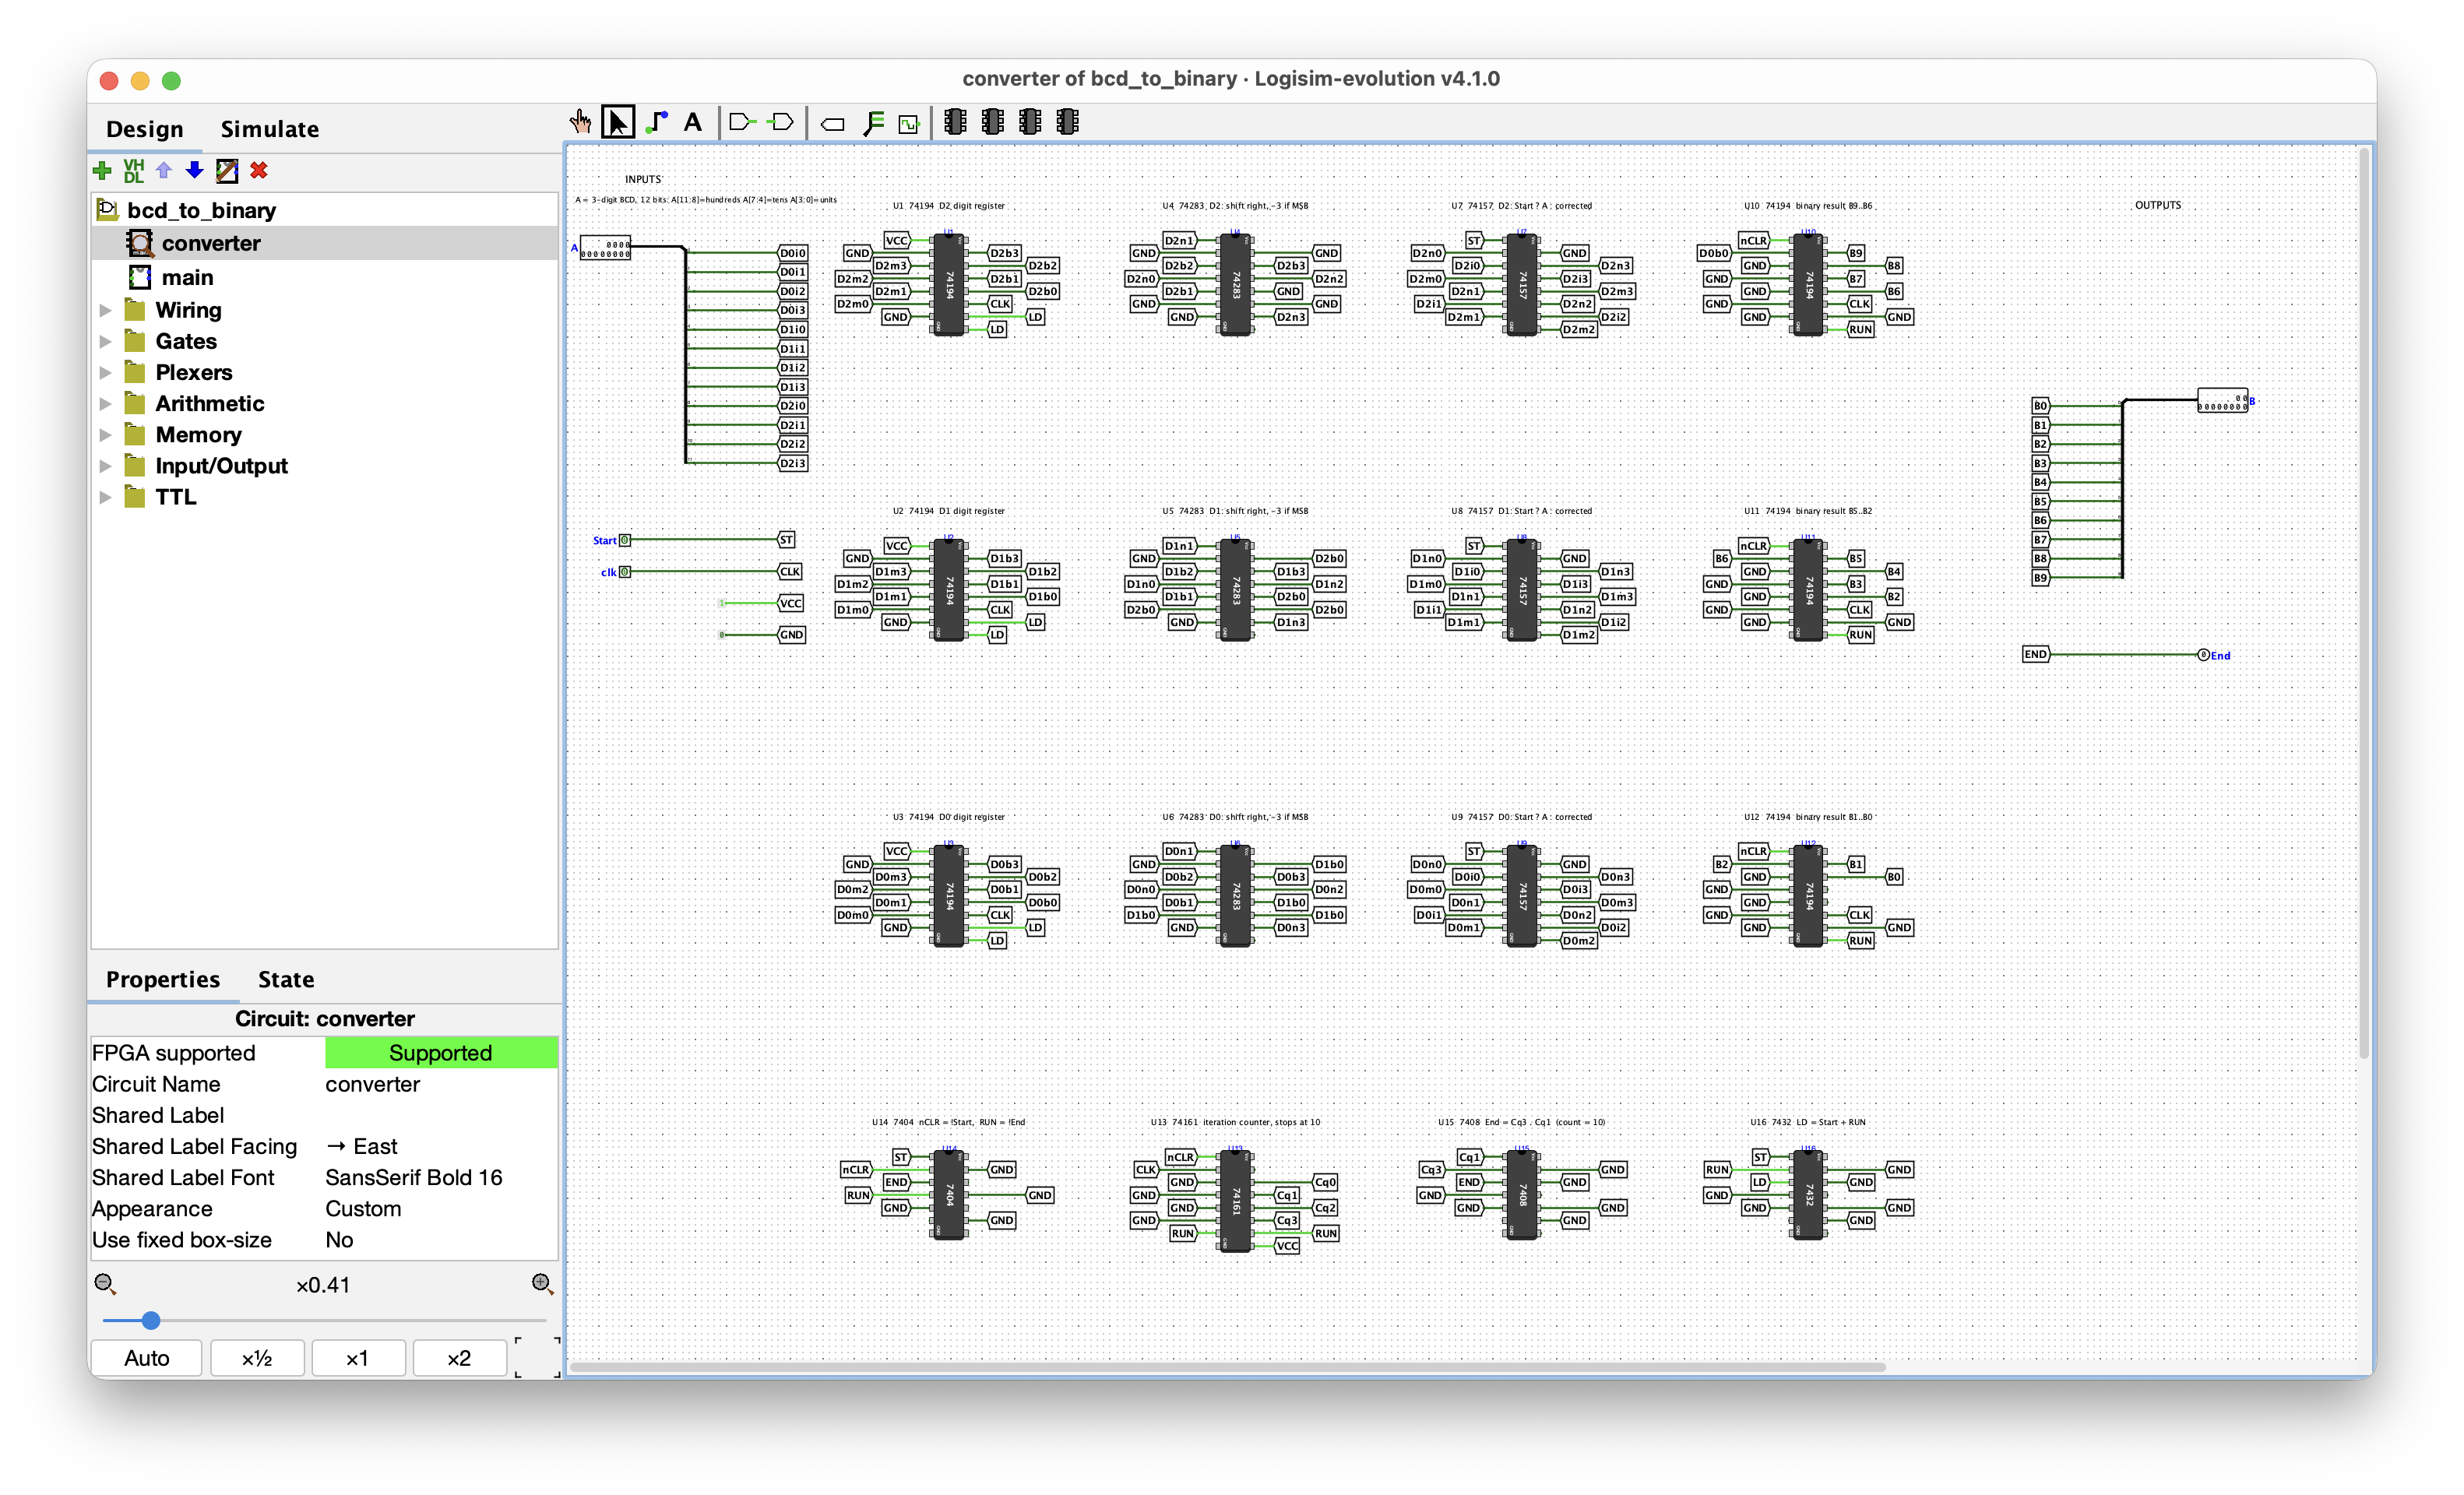
\includegraphics[width=0.95\textwidth]{figs/converter_full.png}
  \caption{نمای کلی مدار \lr{converter} با تمام ۱۶ تراشه}
\end{figure}

\begin{figure}[H]
  \centering
  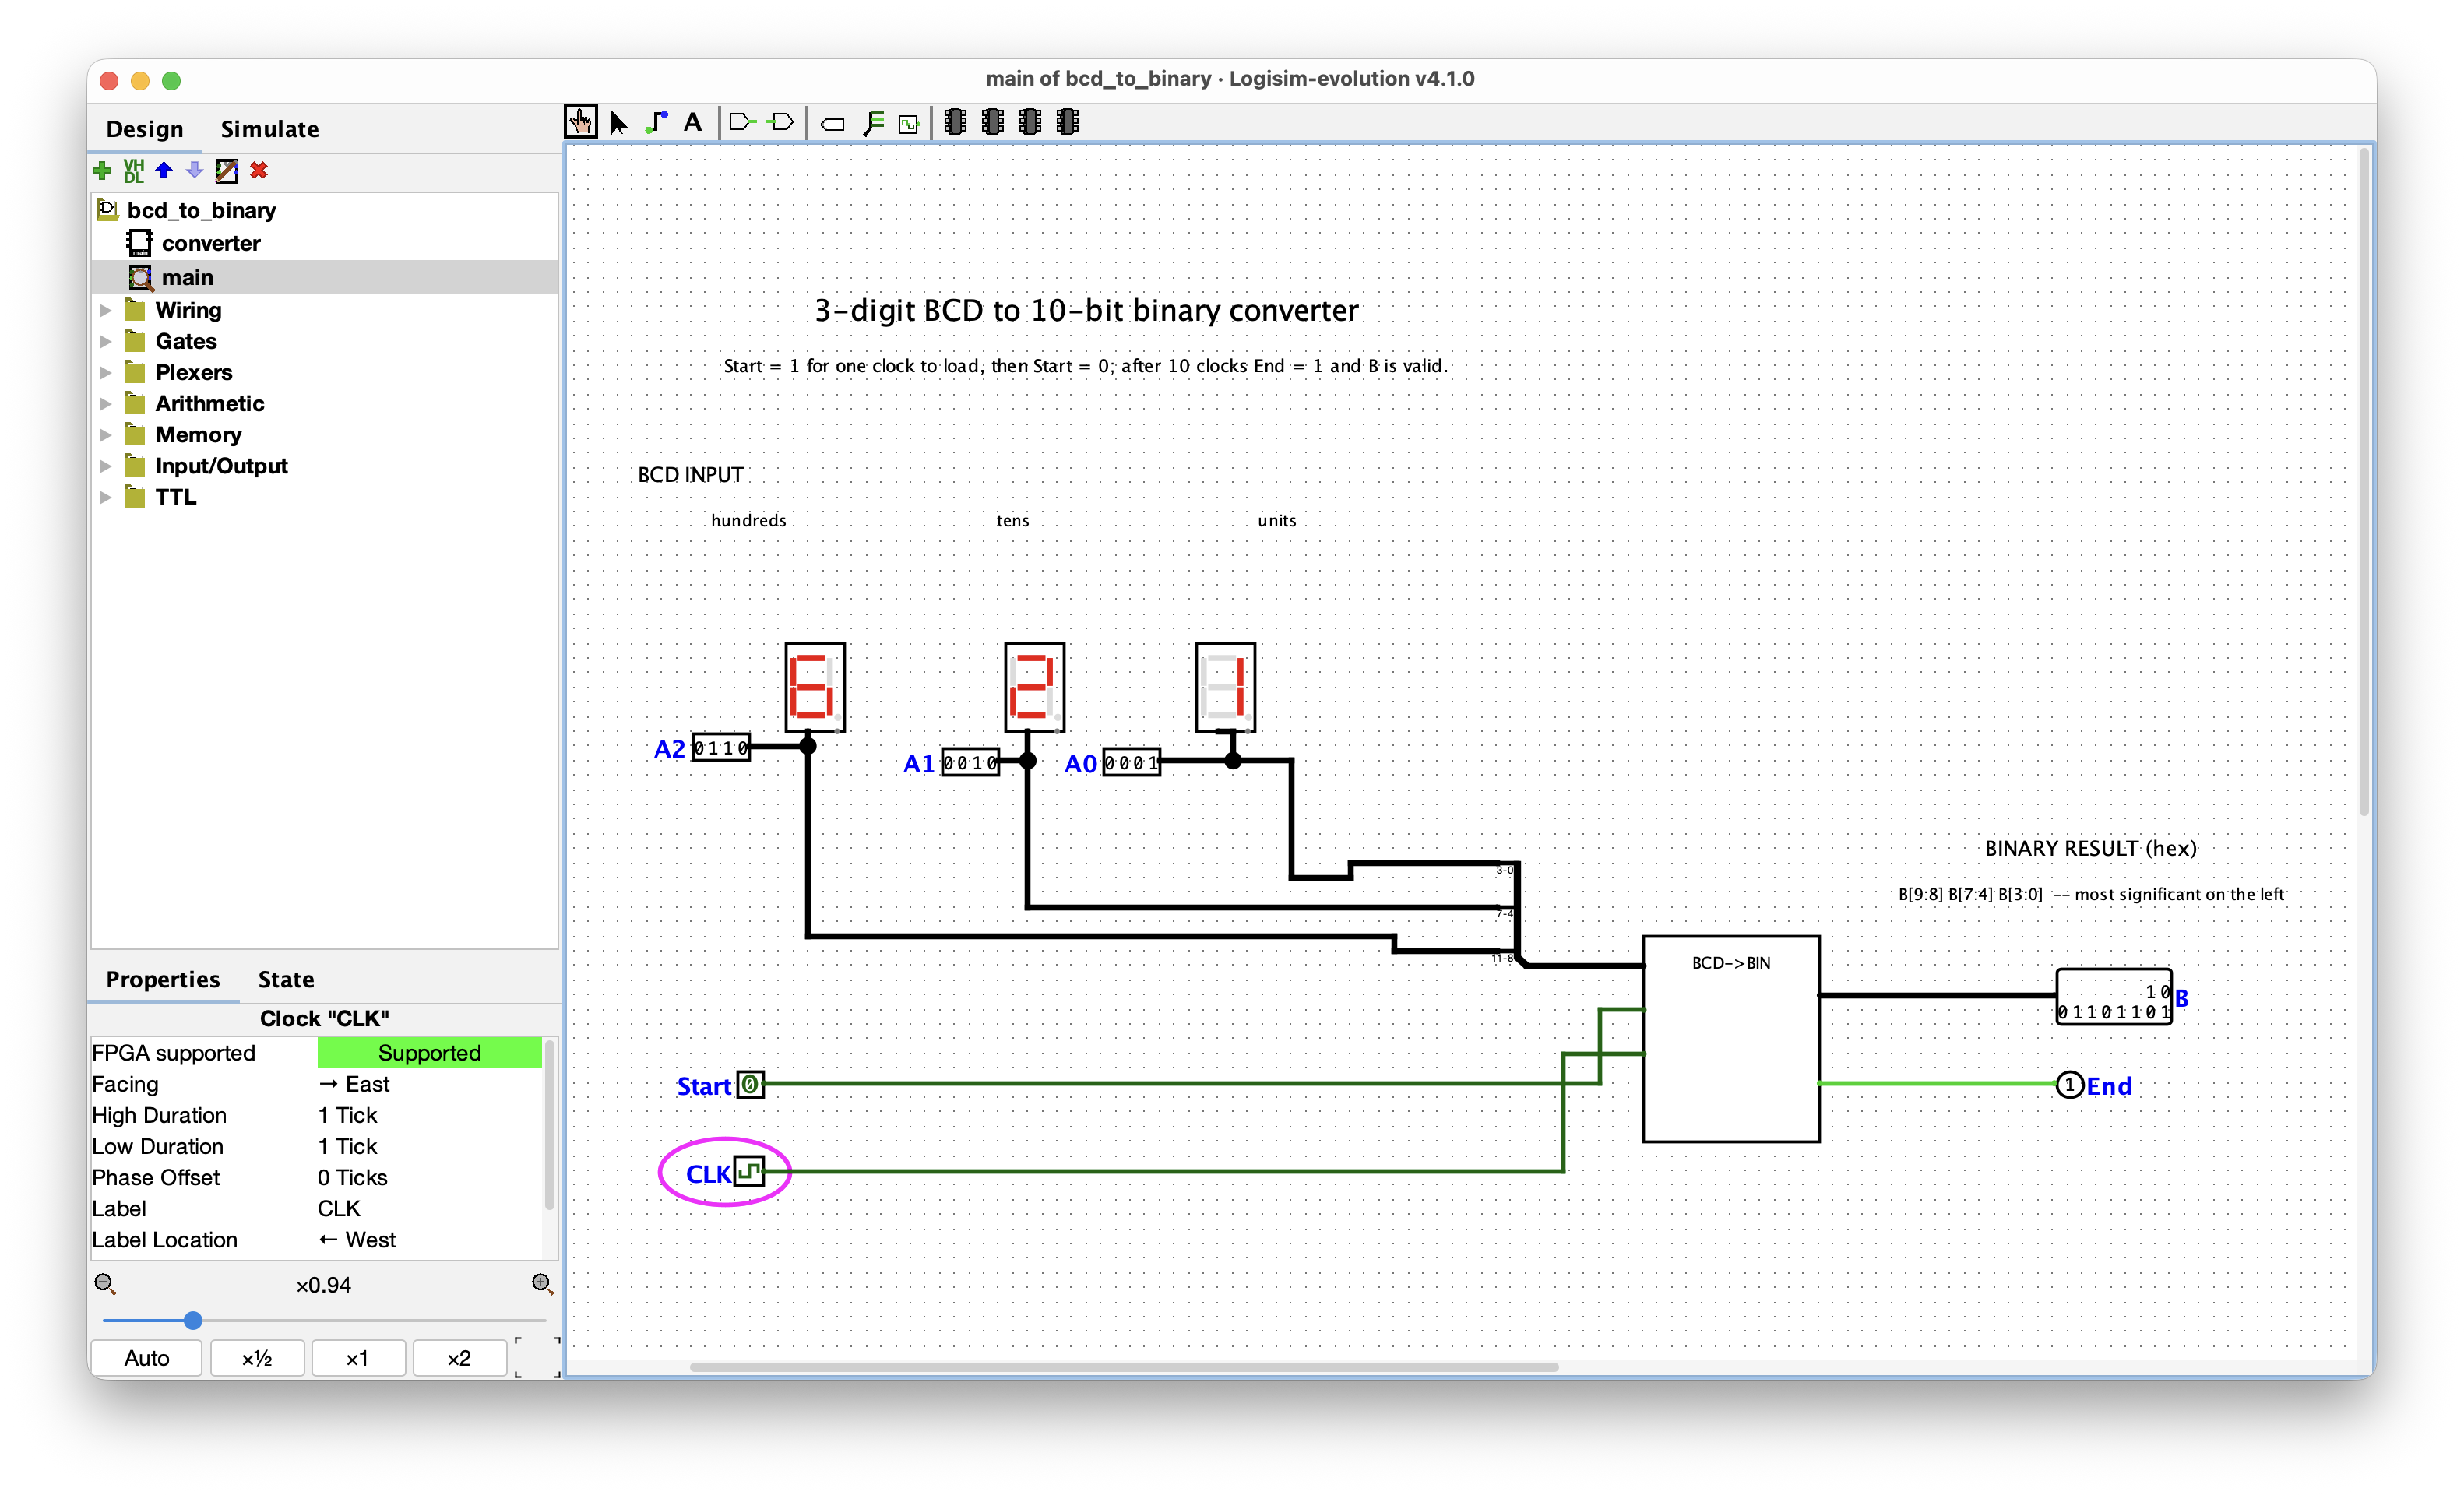
\includegraphics[width=0.95\textwidth]{figs/image.png}
  \caption{مدار \lr{main} با ورودی‌های مجزا}
\end{figure}


نکته: در نوشتن این گزارش و تهیه‌ی جداول از هوش مصنوعی استفاده شده است.


\end{document}
